% !TEX program = lualatex
% Generated by new_lecture_note.sh
\documentclass[11pt]{article}

\usepackage{fontspec}
\usepackage{microtype}
\usepackage{mathtools,amssymb,amsfonts,amsthm,bm}
\usepackage{enumitem}
\usepackage{booktabs,array,xcolor}
\usepackage{geometry,fancyhdr,setspace}
\usepackage{tikz}
\usepackage[hidelinks]{hyperref}
\usepackage[nameinlink,noabbrev]{cleveref}

\geometry{margin=1in,headheight=15pt}
\setstretch{1.12}
\setlength{\parindent}{0pt}
\setlength{\parskip}{0.55em plus 0.12em minus 0.08em}
\setlength{\abovedisplayskip}{0.8em plus 0.2em minus 0.1em}
\setlength{\belowdisplayskip}{0.8em plus 0.2em minus 0.1em}
\allowdisplaybreaks[3]
\setlist{leftmargin=*,topsep=0.35em,itemsep=0.15em,parsep=0pt}

% ---------- Metadata ----------
\newcommand{\studentname}{Keshav Ramamurthy}
\newcommand{\coursename}{Math 118}
\newcommand{\courselongname}{Fourier Analysis}
\newcommand{\lecturenumber}{05}
\newcommand{\lecturetitle}{Lecture 05}
\newcommand{\lecturedate}{\today}

% ---------- Reusable notation ----------
\newcommand{\N}{\mathbb{N}}
\newcommand{\Z}{\mathbb{Z}}
\newcommand{\Q}{\mathbb{Q}}
\newcommand{\R}{\mathbb{R}}
\newcommand{\C}{\mathbb{C}}
\newcommand{\F}{\mathbb{F}}
\newcommand{\K}{\mathbb{K}}
\newcommand{\E}{\mathbb{E}}
\newcommand{\Prob}{\mathbb{P}}
\newcommand{\1}{\mathbf{1}}
\newcommand{\eps}{\varepsilon}
\newcommand{\dd}{\,\mathrm{d}}
\newcommand{\abs}[1]{\left\lvert#1\right\rvert}
\newcommand{\norm}[1]{\left\lVert#1\right\rVert}
\newcommand{\ip}[2]{\left\langle#1,#2\right\rangle}
\newcommand{\set}[1]{\left\{#1\right\}}
\newcommand{\given}{\,\middle\vert\,}
\newcommand{\indep}{\perp\!\!\!\perp}
\newcommand{\lto}{\longrightarrow}
\newcommand{\deriv}[2]{\frac{\mathrm{d}#1}{\mathrm{d}#2}}
\newcommand{\pderiv}[2]{\frac{\partial#1}{\partial#2}}
\DeclareMathOperator{\Aut}{Aut}
\DeclareMathOperator{\Hom}{Hom}
\DeclareMathOperator{\Ker}{ker}
\DeclareMathOperator{\im}{im}
\DeclareMathOperator{\rank}{rank}
\DeclareMathOperator{\range}{range}
\DeclareMathOperator{\nullity}{nullity}
\DeclareMathOperator{\Span}{span}
\DeclareMathOperator{\Var}{Var}
\DeclareMathOperator{\Cov}{Cov}

% ---------- Note environments ----------
\newtheoremstyle{notestyle}{0.7em}{0.7em}{\itshape}{}{}{\bfseries}{.5em}{}
\theoremstyle{notestyle}
\newtheorem{theorem}{Theorem}[section]
\newtheorem{lemma}[theorem]{Lemma}
\newtheorem{proposition}[theorem]{Proposition}
\newtheorem{corollary}[theorem]{Corollary}
\theoremstyle{definition}
\newtheorem{definition}[theorem]{Definition}
\newtheorem{example}[theorem]{Example}
\newtheorem{remark}[theorem]{Remark}
\newenvironment{claim}{\par\noindent\textbf{Claim.}\ }{\par}
\newenvironment{idea}{\par\noindent\textit{Idea.}\ }{\par}
\newenvironment{proofsketch}{\par\noindent\textbf{Proof sketch.}\ }{\par}

% ---------- Header ----------
\pagestyle{fancy}
\fancyhf{}
\fancyhead[L]{\coursename}
\fancyhead[C]{\lecturetitle}
\fancyhead[R]{\studentname}
\fancyfoot[C]{\thepage}

\title{\vspace{-1.5em}\textbf{\coursename\ -- \lecturetitle}}
\author{\studentname}
\date{\lecturedate}

\begin{document}
\maketitle

\section{Main idea}
Just recall an adjoint $A : X \rightarrow Y$ which is a bounded linear operator and an
adjoint is $A^* : Y \rightarrow X$ defined by requiring $$\forall x,y,  \langle Ax, y\rangle_Y =
\langle x, A^* y\rangle_X$$
So basically we are learning about the existence of adjoint etc.

Show $A : X \rightarrow Y$ where $X, Y$ are complete inner product spaces (Hilbert Spaces). has an $adjoint A^*$.
 
\begin{proof}
Given $y \in Y$, $l(x) = \langle Ax, y\rangle$ belongs to $X'.$ 
\par The Riesz Representation Theorem $\exists! v \in X \text{ such that } \forall l(x) =
\langle x, v\rangle$
So 
$$\forall x, \langle Ax, y \rangle = \langle x, A^*y\rangle \iff A^*y = v.$$
\end{proof}
\noindent\textit{Claim.} $A^*$ is a linear operator.
\begin{proof}
    Given $y, z \in Y$ and $\alpha, \beta \in \mathbb{C}$, $$v = A^{*}\left(\alpha y +
        \beta z\right) $$ is the unique vector for which $$\langle Ax, \alpha y + \beta
        z\rangle = \langle x, v\rangle  \text{ } \forall x \in X$$
        Use properties of the inner product on the LHS:
        $$\overline{\alpha}\langle Ax, y\rangle  + \overline{\beta}\langle Ax,
        z\rangle$$
        Then we have $$\overline{\alpha} \langle x, A^* y\rangle +
        \overline{\beta}\langle x, A^* z\rangle $$  which is $$\langle x, \alpha A^* y +
        \beta A^* z\rangle$$
        where v is unique by riesz.
\end{proof}
Properties of the Adjoint:
\begin{itemize}
    \item $(A^*)^* = A$
    \item $(AB)^* = B^*A^*$
    \item $(A^{-1})^{*} = (A^{*})^{-1}$
    \item $\range(A)^{\perp} = \ker(A^{*})$
\end{itemize}
Proof of $(A^*)^*=A$
We have $\forall x \in x, y\in Y, \langle A^*, x\rangle_X = \langle y, Ax \rangle_Y$
\par (Rewrite of our formula)
It is the condition for either $A$ or $A^{*}$ to be the adjoint of the other. 
$$\langle A^{*} y, x\rangle = \langle y, Ax \rangle$$
Conjugate both sides
You get $$x, A^{*} y \rangle = \langle Ax, y\rangle$$
\noindent\textit{Claim.} $||A^*|| = M (M = ||A||)$
First show $||A^{*}|| \le M$, for any $y \in Y$ 
$$||A^{*} y||^2 = \langle A^{*} y , A^{*} y \rangle = \langle y, AA^{*} y\rangle$$
Use Cauchy:
$\langle y, AA^{*}y\rangle \le ||y|| cdot ||AA^{*}|| \cdot ||A^{*} y||$
\par If $A^{*}y \ne 0$, divide 
$$||A^{*}y || \le M||y||$$
which is true for every y, and the zero ase is also true.
\par Use $(A^{*})^{*}= A$ to conclude and basically want to show $||A|| \le ||A^{*}||$
You can write it as $$||Ax||^2 = \langle Ax, Ax \rangle =\langle x, A* Ax\rangle \le
||x||\cdot ||A^{*}Ax || \le ||x|| \cdot ||A^{*}|| \cdot ||Ax||$$
To proof that $\range(A)^{\perp} = \ker(A^{*})$
$$y \in \range(A)^{\perp} \iff \forall x \in X, \langle Ax, y\rangle = 0$$
Which is analogous to $$\forall x \in X, \langle x, A^* y \rangle = 0 \iff A^{*}y = 0$$
\textit{Write the one-sentence point of today's lecture here.}
\section{Projections Pt 2.}
We define $P : V\rightarrow V$ to be a projection if $P$ is bounded and $P^2 = P$ (as an
operator), where $P^2$ means composition: $P^2(x) = P(P(x))$.
So $P^2 = P$ says applying $P$ a second time does nothing new --- think of projecting a
point onto the floor: once you are on the floor, projecting again does not move you.
(For example, $P(x, y) = (x, 0)$ satisfies $P(P(x,y)) = (x,0) = P(x,y)$.)
\par $I - P$ keeps whatever $P$ threw away, so it should also be a projection.
\noindent\textit{Claim.} If $P$ is a projection, so is $I - P$
\begin{proof}
    $$(I - P)^2 = (I - P  - P + P^2) = (I - P) + (P^2 - P) = (I - P)$$
\end{proof}
This is just the binomial expansion (legal since $I$ commutes with everything), and the
last step uses exactly the hypothesis: $P^2 - P = 0$.

\begin{center}
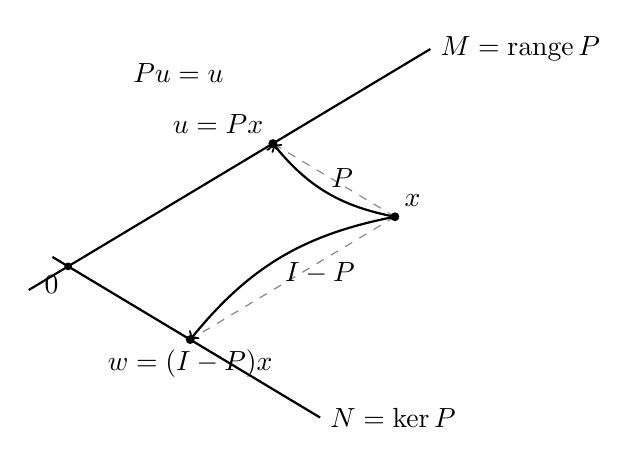
\begin{tikzpicture}
  % complementary subspaces through the origin
  \draw[thick] (-0.5,-0.3) -- (4.6,2.76) node[right] {$M = \range P$};
  \draw[thick] (-0.2,0.12) -- (3.2,-1.92) node[right] {$N = \ker P$};
  % the point x and its decomposition
  \coordinate (x) at (4.15,0.63);
  \coordinate (u) at (2.6,1.56);
  \coordinate (w) at (1.55,-0.93);
  \draw[dashed,gray] (x) -- (u);
  \draw[dashed,gray] (x) -- (w);
  \fill (x) circle (1.6pt) node[above right] {$x$};
  \fill (u) circle (1.6pt) node[above left] {$u = Px$};
  \fill (w) circle (1.6pt) node[below] {$w = (I-P)x$};
  \fill (0,0) circle (1.4pt) node[below left] {$0$};
  % P keeps the M-part, I-P keeps the N-part
  \draw[->,thick] (x) to[bend left=20] node[above right=-2pt] {$P$} (u);
  \draw[->,thick] (x) to[bend right=20] node[below right=-2pt] {$I-P$} (w);
  % idempotence: a second pass does nothing
  \draw[->,thick] (u) to[out=120,in=60,looseness=6] (u);
  \node at (1.4,2.45) {$Pu = u$};
\end{tikzpicture}
\end{center}

So $P$ keeps $\range P = M$ and kills $\ker P = N$, while $I - P$ does the
reverse, splitting $V = \range P \oplus \ker P$ into the two complementary pieces.

\noindent\textit{Claim.} For an orthogonal projection ($P^2 = P$ and $P^* = P$), we have
$(I - P)u \perp Pv$ for all $u, v \in V$.
\begin{proof}
    Using $\langle Ax, y\rangle = \langle x, A^{*}y\rangle$ with $P^{*} = P$,
    $$\langle (I-P)u,\; Pv\rangle = \langle P(I-P)u,\; v\rangle = \langle (P - P^2)u,\; v\rangle = 0,$$
    since $P(I - P) = P - P^2 = 0$.
\end{proof}
\par This is exactly what ``orthogonal'' adds: a general projection only makes
$\range P$ and $\ker P$ complementary (the two lines in the diagram, possibly
skew); $P^* = P$ is what makes them perpendicular. Conversely, if $(I-P)u \perp Pv$ for
all $u, v$, then taking $u \in \ker P$ (so $(I-P)u = u$) gives $\ker P \perp
\range P$, so $P$ is the orthogonal projection onto its range.

\par \textbf{Introduction: projecting without an orthonormal basis.}
We started from the orthonormal case: if $\set{e_1, \dots, e_N}$ is an orthonormal basis
for $V_0$, then
$$Pu = \sum_{n=1}^{N} \ip{u}{e_n}\, e_n$$
is the orthogonal projection onto $V_0$.
Now let $\varphi_1, \dots, \varphi_N$ be a basis for $V_0$ that is \emph{not}
orthonormal. The coefficients are no longer just the inner products $\ip{u}{\varphi_n}$
--- so how do we project without running Gram--Schmidt?
\par The idea: since $Pu$ lands in $V_0$, it must be some combination
$$Pu = c_1 \varphi_1 + c_2 \varphi_2 + \cdots + c_N \varphi_N$$
with unknown numbers $c_1, \dots, c_N$ --- that is $N$ unknowns, so we need $N$
equations. The projection condition is that $u - Pu$ is perpendicular to every vector in
$V_0$, and it is enough to check it against the basis vectors:
$$\ip{u - Pu}{\varphi_n} = 0 \qquad \text{for } n = 1, \dots, N.$$
Expanding $Pu$ and rearranging,
$$c_1 \ip{\varphi_1}{\varphi_n} + c_2 \ip{\varphi_2}{\varphi_n} + \cdots +
c_N \ip{\varphi_N}{\varphi_n} = \ip{u}{\varphi_n},
\qquad n = 1, \dots, N.$$
That is an ordinary $N \times N$ linear system --- solve it with Gaussian elimination,
like any system from linear algebra. The matrix is all the pairwise inner products of
the $\varphi$'s (it is called the \textit{Gram matrix}); the right side is the inner
products of $u$ with each $\varphi_n$.

\par \textbf{The Gram matrix, from scratch.} Given vectors $\varphi_1, \dots,
\varphi_N$, their \textit{Gram matrix} $G$ is the $N \times N$ table of all their
pairwise inner products:
$$G_{mn} = \ip{\varphi_m}{\varphi_n}, \qquad m, n = 1, \dots, N.$$
That is the whole definition --- row $m$, column $n$ holds the inner product of
$\varphi_m$ with $\varphi_n$. What the table contains:
\begin{itemize}
    \item \textbf{Diagonal entries:} $G_{nn} = \ip{\varphi_n}{\varphi_n} =
    \norm{\varphi_n}^2$ --- the squared length of each basis vector.
    \item \textbf{Off-diagonal entries:} for real vectors,
    $\ip{\varphi_m}{\varphi_n} = \norm{\varphi_m}\, \norm{\varphi_n} \cos\theta$ ---
    they record the angle between $\varphi_m$ and $\varphi_n$, and they are $0$ exactly
    when the two vectors are perpendicular.
    \item $G = I$ exactly when the basis is orthonormal (all lengths $1$, all angles
    $90^{\circ}$).
    \item $G$ is always Hermitian: $G_{nm} = \overline{G_{mn}}$; for real vectors it is
    simply symmetric.
\end{itemize}
\par \textbf{Two small examples.} For $\varphi_1 = (1,0)$, $\varphi_2 = (1,1)$ in
$\R^2$:
$$G = \begin{pmatrix} \ip{\varphi_1}{\varphi_1} & \ip{\varphi_1}{\varphi_2} \\
\ip{\varphi_2}{\varphi_1} & \ip{\varphi_2}{\varphi_2} \end{pmatrix}
= \begin{pmatrix} 1 & 1 \\ 1 & 2 \end{pmatrix}.$$
For the functions $1, t, t^2$ on $[0,1]$, the entries are integrals --- for example
$\ip{t}{t^2} = \int_0^1 t \cdot t^2 \dd t = \frac{1}{4}$ and
$\ip{t^2}{t^2} = \int_0^1 t^4 \dd t = \frac{1}{5}$ --- which gives
$$G = \begin{pmatrix}
1 & \tfrac{1}{2} & \tfrac{1}{3} \\
\tfrac{1}{2} & \tfrac{1}{3} & \tfrac{1}{4} \\
\tfrac{1}{3} & \tfrac{1}{4} & \tfrac{1}{5}
\end{pmatrix}.$$
\par One identity worth remembering: expanding a squared norm with linearity,
$$\norm{c_1\varphi_1 + \cdots + c_N\varphi_N}^2
= \sum_{m,n=1}^{N} c_m\, G_{mn}\, \overline{c_n}.$$
The Gram matrix is exactly the thing that turns a coefficient combination into a
squared norm --- which is why it is the coefficient matrix of the projection system,
and why that system always has a unique solution when the $\varphi$'s form a basis:
the right side above is a norm, so it is $0$ only when every $c_n = 0$.

\par Sanity check: if the $\varphi_n$ \emph{were} orthonormal, the matrix would be the
identity and we would get $c_n = \ip{u}{\varphi_n}$ --- exactly the formula we started
from.

\par \textbf{A tiny example.} In $\R^3$, take $V_0 = \Span\set{\varphi_1, \varphi_2}$ with
$\varphi_1 = (1,0,0)$, $\varphi_2 = (1,1,0)$ (this is the $xy$-plane, but the basis is
not orthonormal), and $u = (1,2,3)$. The pairwise inner products are
$$\ip{\varphi_1}{\varphi_1} = 1, \qquad
\ip{\varphi_1}{\varphi_2} = 1, \qquad \ip{\varphi_2}{\varphi_2} = 2,$$
and $\ip{u}{\varphi_1} = 1$, $\ip{u}{\varphi_2} = 3$. So the system reads
$$\begin{cases} c_1 + \phantom{2}c_2 = 1 \\ c_1 + 2c_2 = 3 \end{cases}
\implies c_2 = 2, \; c_1 = -1,$$
and $Pu = -\varphi_1 + 2\varphi_2 = (1,2,0)$ --- the usual projection of $(1,2,3)$ onto
the $xy$-plane, as expected. But notice $c_2 = 2$ while $\ip{u}{\varphi_2} = 3$: with a
non-orthonormal basis the coefficients are \emph{not} the inner products.

\par \textbf{Functions work the same way.} If $V_0$ is spanned by functions, say
$\varphi_1 = 1$, $\varphi_2 = t$, $\varphi_3 = t^2$ on $[0,1]$, nothing changes except
how you compute inner products --- for functions they are integrals:
$$\ip{f}{g} = \int_0^1 f(t)\, \overline{g(t)}\, \dd t.$$
So the matrix entries are numbers like
$$\ip{\varphi_1}{\varphi_1} = \int_0^1 1\, \dd t = 1, \qquad
\ip{\varphi_2}{\varphi_1} = \int_0^1 t\, \dd t = \frac{1}{2}, \qquad
\ip{\varphi_3}{\varphi_2} = \int_0^1 t^3\, \dd t = \frac{1}{4},$$
and the right side is $\ip{u}{1}$, $\ip{u}{t}$, $\ip{u}{t^2}$ (integrals of $u$ against
each basis function). Solve the system, combine the $\varphi$'s with those
coefficients, and that is the projection --- no Gram--Schmidt needed.
\section{Definitions and notation}
\begin{definition}[First definition]
Write the definition and one sentence explaining why it matters.
\end{definition}

\section{Claims, theorems, and proof sketches}
\begin{claim}
State the claim in one precise sentence.
\end{claim}

\begin{proofsketch}
Record the key idea, the first useful equation, and the step that still needs checking.
\end{proofsketch}

\section{Examples and calculations}
\begin{example}[Lecture example]
Write the setup, the calculation, and the conclusion.
\end{example}

\section{Questions and follow-up}
\begin{itemize}
  \item What is still unclear?
  \item Which exercise or reading should I revisit?
  \item TODO:
\end{itemize}

\end{document}
